\documentclass{beamer}
\usepackage{amsmath}
\usepackage{hyperref}
\usepackage{listings}
\usepackage{xcolor}
\hypersetup{colorlinks=true, citecolor=blue, filecolor=blue, linkcolor=blue, urlcolor=blue}
\definecolor{codegreen}{rgb}{0,0.6,0}
\definecolor{codegray}{rgb}{0.5,0.5,0.5}
\definecolor{codepurple}{rgb}{0.58,0,0.82}
\definecolor{backcolour}{rgb}{0.95,0.95,0.92}
 
\lstdefinestyle{mystyle}{
    backgroundcolor=\color{backcolour},   
    commentstyle=\color{codegreen},
    keywordstyle=\color{magenta},
    numberstyle=\tiny\color{codegray},
    stringstyle=\color{codepurple},
    basicstyle=\ttfamily\footnotesize,
    breakatwhitespace=false,         
    breaklines=true,                 
    captionpos=b,                    
    keepspaces=true,                 
    %numbers=left,                    
    numbersep=5pt,                  
    showspaces=false,                
    showstringspaces=false,
    showtabs=false,                  
    tabsize=2
}
 
\lstset{style=mystyle}

\mode<presentation> {

% The Beamer class comes with a number of default slide themes
% which change the colors and layouts of slides. Below this is a list
% of all the themes, uncomment each in turn to see what they look like.

%\usetheme{default}
\usetheme{AnnArbor}
%\usetheme{Antibes}
%\usetheme{Bergen}
%\usetheme{Berkeley}
%\usetheme{Berlin}
%\usetheme{Boadilla}
%\usetheme{CambridgeUS}
%\usetheme{Copenhagen}
%\usetheme{Darmstadt}
%\usetheme{Dresden}
%\usetheme{Frankfurt}
%\usetheme{Goettingen}
%\usetheme{Hannover}
%\usetheme{Ilmenau}
%\usetheme{JuanLesPins}
%\usetheme{Luebeck}
%\usetheme{Madrid}
%\usetheme{Malmoe}
%\usetheme{Marburg}
%\usetheme{Montpellier}
%\usetheme{PaloAlto}
%\usetheme{Pittsburgh}
%\usetheme{Rochester}
%\usetheme{Singapore}
%\usetheme{Szeged}
%\usetheme{Warsaw}

% As well as themes, the Beamer class has a number of color themes
% for any slide theme. Uncomment each of these in turn to see how it
% changes the colors of your current slide theme.

%\usecolortheme{albatross}
%\usecolortheme{beaver}
%\usecolortheme{beetle}
%\usecolortheme{crane}
%\usecolortheme{dolphin}
%\usecolortheme{dove}
%\usecolortheme{fly}
%\usecolortheme{lily}
%\usecolortheme{orchid}
%\usecolortheme{rose}
%\usecolortheme{seagull}
%\usecolortheme{seahorse}
%\usecolortheme{whale}
\usecolortheme{wolverine}

%\setbeamertemplate{footline} % To remove the footer line in all slides uncomment this line
\setbeamertemplate{footline}[page number] % To replace the footer line in all slides with a simple slide count uncomment this line

\setbeamertemplate{navigation symbols}{} % To remove the navigation symbols from the bottom of all slides uncomment this line
}

\usepackage{graphicx} % Allows including images
\usepackage{booktabs} % Allows the use of \toprule, \midrule and \bottomrule in tables
%\usepackage {tikz}
\usepackage{tkz-graph}
\GraphInit[vstyle = Shade]
\tikzset{
  LabelStyle/.style = { rectangle, rounded corners, draw,
                        minimum width = 2em, fill = yellow!50,
                        text = red, font = \bfseries },
  VertexStyle/.append style = { inner sep=5pt,
                                font = \normalsize\bfseries},
  EdgeStyle/.append style = {->, bend left} }
\usetikzlibrary {positioning}
%\usepackage {xcolor}
\definecolor {processblue}{cmyk}{0.96,0,0,0}
%----------------------------------------------------------------------------------------
%	TITLE PAGE
%----------------------------------------------------------------------------------------

\title[Gradient Descent]{Numerical Optimization 06: 1st order methods} %

\author{Qiang Zhu} % Your name
\institute[University of Nevada Las Vegas] % Your institution as it will appear on the bottom of every slide, may be shorthand to save space
{
University of Nevada Las Vegas\\ % Your institution for the title page
\medskip
}
\date{\today} % Date, can be changed to a custom date

\begin{document}

\begin{frame}
\titlepage % Print the title page as the first slide
\end{frame}

\begin{frame}
\frametitle{Overview} % Table of contents slide, comment this block out to remove it
\tableofcontents % Throughout your presentation, if you choose to use \section{} and \subsection{} commands, these will automatically be printed on this slide as an overview of your presentation
\end{frame}

%----------------------------------------------------------------------------------------
%	PRESENTATION SLIDES
%----------------------------------------------------------------------------------------

%------------------------------------------------
\section{Gradient methods with fixed learning rate}
\begin{frame}{Gradient methods with fixed learning rate}
We have talked about steepest descent and conjugate gradient methods, which usually work with the line search methods. Alternatively, it is popular to use the fixed learning rate method based on Gradient descent. However, the standard version will take a long time to traverse a nearly flat surface.
Several methods have been proposed. They are commonly used in machine learning neural networks training.
\begin{columns}
\begin{column}{.4\textwidth}
\begin{itemize}
    \item Momentum
    \item Nesterov Momentum
    \item Adagrad
    \item RMSProp
    \item Adadelta
    \item Adam
\end{itemize}
\end{column}

\begin{column}{.6\textwidth}
\begin{figure}
\centering
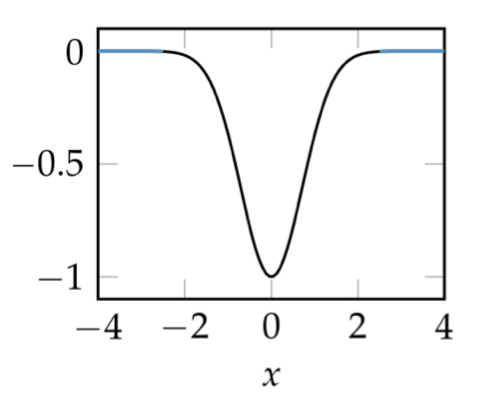
\includegraphics[width=60mm]{Figs/flat.jpeg}
\end{figure}
\end{column}
\end{columns}
\end{frame}



\section{Momentum}
\begin{frame}{Momentum}
Allowing momentum to accumulate is one way to speed the progress. 
Thus we can modify the gradient descent to incorporate momentum.
\begin{gather*}
    \boldsymbol{v}^{k+1} = \beta \boldsymbol{v}^k + \alpha \boldsymbol{g}^k \\
    \boldsymbol{x}^{k+1} = \boldsymbol{x}^k + \boldsymbol{v}^{k+1} 
\end{gather*}
When $\beta$=0, it is gradient descent. 
\begin{figure}
\centering
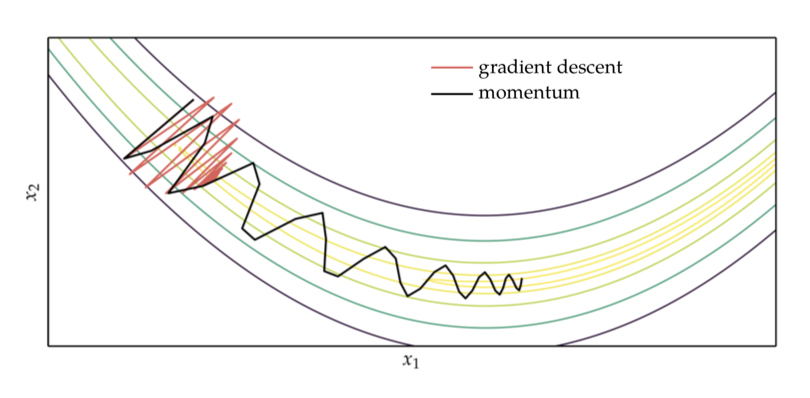
\includegraphics[width=100mm]{Figs/momentum.jpeg}
\end{figure}


\end{frame}

\section{Nesterov Momentum}
\begin{frame}{Nesterov Momentum}
One issue of momentum is that the steps do not slow down enough at the bottom of a valley and it tends to \textcolor{blue}{overshoot the valley}. Nesterov Momentum remedies the issue by the following updates,
\begin{gather*}
    \boldsymbol{v}^{k+1} = \beta \boldsymbol{v}^k + \alpha \nabla f(\boldsymbol{x} + \beta \boldsymbol{v}^k) \\
    \boldsymbol{x}^{k+1} = \boldsymbol{x}^k + \boldsymbol{v}^{k+1} 
\end{gather*}

\begin{figure}
\centering
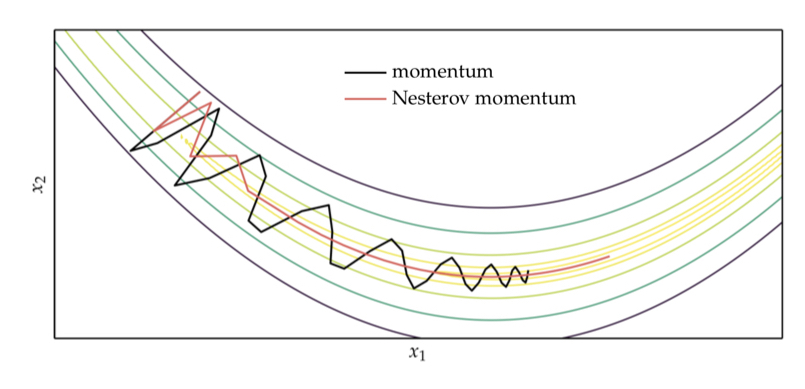
\includegraphics[width=100mm]{Figs/n-momentum.jpeg}
\end{figure}

\end{frame}

\section{Adagrad}
\begin{frame}{Adagrad}
Momentum and Nesterov Momentum update all componens of $x$ with the same learning rate. The adaptive subgradient method (Adagrad), adapts a learning rate for each one in x.
\begin{gather*}
    x_i^{k+1} = x_i^k - \frac{\alpha}{\epsilon + \sqrt{s_i^k}} g^k \\
    s_i^k = \sum_{j=1}^k \bigg(g_i^j\bigg)^2 
\end{gather*}
where $\epsilon$ is a small value on the order of 1e-8, to prevent the case of division by zero. 
Adagrad is far less sensitive to the learning rate $\alpha$. 
\end{frame}

\section{RMSProp and Adadelta}
\begin{frame}{RMSProp and Adadelta}

In Adagrad, the learning rate may monotonically decrease. To prevent this, \textcolor{blue}{RMPprop} maintains a decaying average of squared gradients.
\begin{equation*}
    \boldsymbol{s}^{k+1} = \gamma \boldsymbol{s}^k + (1-\gamma)(\boldsymbol{g}^k \odot \boldsymbol{g}^k)
\end{equation*}

where $\gamma$ is between 0 and 1, and usually is 0.9.

\begin{equation*}
\begin{split}
    x_i^{k+1} &= x_i^k - \frac{\alpha}{\epsilon + \sqrt{s_i^k}} g_i^k \\
              &= x_i^k - \frac{\alpha}{\epsilon + \textrm{RMS}(g_i)} g_i^k        
\end{split}
\end{equation*}

While in \textcolor{blue}{Adadelta}, an exponentially decaying average is used,

\begin{equation*}
    x_i^{k+1} = x_i^k - \frac{\textrm{RMS}(\delta x_i)}{\epsilon + \textrm{RMS}(g_i)} g_i^k        
\end{equation*}

\end{frame}

\section{Adam}
\begin{frame}{Adam}

The adaptive moment estimation (Adam) is so far the most widely used optimization method in neural network training.
It stores both an exponentially decaying squared gradient like RMSProp and Adadelta, but also an exponentially decaying gradient like momentum.
\begin{equation*}
 \begin{split}
    \boldsymbol{v}^{k+1} &= \gamma_v \boldsymbol{v}^k + (1-\gamma_v) \boldsymbol{g}^k \\
    \boldsymbol{s}^{k+1} &= \gamma_s \boldsymbol{s}^k + (1-\gamma_s) \bigg(\boldsymbol{g}^k \odot \boldsymbol{g}^k \bigg)\\
    \hat{\boldsymbol{v}}^{k+1} &= \boldsymbol{v}^{k+1}/(1-\gamma_v^k)\\
    \hat{\boldsymbol{s}}^{k+1} &= \boldsymbol{s^{k+1}}/(1-\gamma_s^k)\\
    \boldsymbol{x}^{k+1} &= \boldsymbol{x}^k - \alpha \hat{\boldsymbol{v}}^{k+1}/\bigg(\epsilon + \sqrt{\hat{\boldsymbol{s}}^{k+1}}\bigg)
 \end{split}
\end{equation*}


\end{frame}


\section{Summary}
\begin{frame}{Summary}
    \begin{itemize}
        \item Descent methods with momentum build up progress in favorable directions
        \item A wide variety of accelerated descent methods use special techniques to speed up descent
    \end{itemize}
\end{frame}
\end{document}

